\documentclass[10pt]{article}
\usepackage[margin=1in]{geometry}
\usepackage[T1]{fontenc}
\usepackage{lmodern}
\usepackage{microtype}
\usepackage{amsmath,amssymb}
\usepackage{graphicx}
\usepackage{booktabs}
\usepackage{xcolor}
\usepackage{caption}
\usepackage{enumitem}
\usepackage{titlesec}
\usepackage[colorlinks=true,linkcolor=black,citecolor=black,urlcolor=blue!50!black]{hyperref}
\captionsetup{font=small,labelfont=bf}
\setlist{nosep,leftmargin=1.4em}
\titlespacing*{\section}{0pt}{1.1ex plus .3ex}{.5ex}
\titlespacing*{\subsection}{0pt}{.9ex plus .2ex}{.3ex}
\titleformat*{\subsection}{\normalsize\bfseries}
\setlength{\parskip}{.35ex plus .2ex}
\setlength{\textfloatsep}{8pt plus 2pt}
% generated by scripts/make_tex.py from out/numbers.json; do not edit
\newcommand{\nForecasts}{2,337,011}
\newcommand{\nForecastsM}{2.34}
\newcommand{\nForecastsDataset}{2,095,241}
\newcommand{\nForecastsMarket}{241,770}
\newcommand{\nItems}{43,303}
\newcommand{\nItemsDataset}{39,198}
\newcommand{\nItemsMarket}{4,105}
\newcommand{\nQuestions}{4,781}
\newcommand{\nQuestionsDataset}{2,607}
\newcommand{\nRounds}{37}
\newcommand{\nListed}{649}
\newcommand{\nCand}{207}
\newcommand{\nCandWide}{374}
\newcommand{\nFilesDropped}{425}
\newcommand{\nBoot}{1,000}
\newcommand{\nSplits}{400}
\newcommand{\reproMatched}{316}
\newcommand{\reproPublished}{506}
\newcommand{\reproRhoOverall}{0.985}
\newcommand{\reproRhoDataset}{0.967}
\newcommand{\reproRhoMarket}{0.999}
\newcommand{\reproMadDataset}{0.006}
\newcommand{\reproMadMarket}{0.0002}
\newcommand{\reproMadOverall}{0.003}
\newcommand{\superPubOverall}{0.101}
\newcommand{\superOursOverall}{0.098}
\newcommand{\oedSuperUni}{49 (42 to 56)}
\newcommand{\vSuperUni}{49}
\newcommand{\oedSuperPre}{62 (56 to 69)}
\newcommand{\vSuperPre}{62}
\newcommand{\oedSuperHigh}{22 (4 to 35)}
\newcommand{\vSuperHigh}{22}
\newcommand{\oedSuperEven}{48 (40 to 56)}
\newcommand{\vSuperEven}{48}
\newcommand{\oedPublicUni}{31 (23 to 38)}
\newcommand{\vPublicUni}{31}
\newcommand{\oedPublicPre}{34 (27 to 40)}
\newcommand{\vPublicPre}{34}
\newcommand{\oedPublicHigh}{8 ($-$2 to 16)}
\newcommand{\vPublicHigh}{8}
\newcommand{\oedPublicEven}{33 (21 to 44)}
\newcommand{\vPublicEven}{33}
\newcommand{\oedBestUni}{44 (41 to 48)}
\newcommand{\vBestUni}{44}
\newcommand{\vMedUni}{20}
\newcommand{\linkDiffUni}{0.05 (95\% CI $-$0.02 to 0.12)}
\newcommand{\linkPUni}{90.5}
\newcommand{\oedBestPre}{53 (48 to 57)}
\newcommand{\vBestPre}{53}
\newcommand{\vMedPre}{26}
\newcommand{\linkDiffPre}{0.09 (95\% CI 0.02 to 0.17)}
\newcommand{\linkPPre}{99.7}
\newcommand{\oedBestHigh}{29 (25 to 34)}
\newcommand{\vBestHigh}{29}
\newcommand{\vMedHigh}{6}
\newcommand{\linkDiffHigh}{$-$0.07 (95\% CI $-$0.25 to 0.06)}
\newcommand{\linkPHigh}{17.1}
\newcommand{\oedBestEven}{41 (36 to 46)}
\newcommand{\vBestEven}{41}
\newcommand{\vMedEven}{18}
\newcommand{\linkDiffEven}{0.07 (95\% CI $-$0.02 to 0.15)}
\newcommand{\linkPEven}{94.4}
\newcommand{\shareNonposHigh}{31}
\newcommand{\shareNonposUni}{6}
\newcommand{\rhoPre}{0.96}
\newcommand{\rhoHigh}{0.85}
\newcommand{\rhoEven}{0.98}
\newcommand{\moveHigh}{19}
\newcommand{\movePre}{9}
\newcommand{\keepHigh}{13}
\newcommand{\keepPre}{16}
\newcommand{\peakTheta}{0.23}
\newcommand{\peakValue}{36}
\newcommand{\medAtLow}{3}
\newcommand{\medAtHigh}{0.4}
\newcommand{\medAtHalf}{16}
\newcommand{\medAtFive}{12}
\newcommand{\medAtNinety}{2}
\newcommand{\nonposLow}{44}
\newcommand{\nonposMid}{2}
\newcommand{\nonposHigh}{49}
\newcommand{\bestAtLow}{38}
\newcommand{\bestAtHigh}{26}
\newcommand{\beatPriceShare}{1.9}
\newcommand{\beatPriceCount}{4}
\newcommand{\beatPriceMax}{2.9}
\newcommand{\priceValue}{54}
\newcommand{\medMarketValue}{32}
\newcommand{\medDatasetValue}{18}
\newcommand{\rhoBMid}{0.94}
\newcommand{\rhoOMid}{0.96}
\newcommand{\rhoBNinety}{0.64}
\newcommand{\rhoONinety}{0.88}
\newcommand{\rhoBNinetyFive}{0.55}
\newcommand{\rhoONinetyFive}{0.83}
\newcommand{\rhoBNinetyWide}{0.57}
\newcommand{\rhoONinetyWide}{0.81}
\newcommand{\pickB}{15}
\newcommand{\pickO}{25}
\newcommand{\pickDiff}{10 points (middle 95\% of splits: 6 to 14)}
\newcommand{\pickPOwn}{100}
\newcommand{\pickDiffWide}{9 points (4 to 14)}
\newcommand{\rhoBMarket}{0.88}
\newcommand{\rhoOMarket}{0.85}
\newcommand{\brierWinsOverall}{12}
\newcommand{\brierWinsMarket}{13}
\newcommand{\nSelThetas}{15}
\newcommand{\selPreB}{52}
\newcommand{\selPreO}{52}
\newcommand{\selHighB}{28}
\newcommand{\selHighO}{29}
\newcommand{\selEvenB}{40}
\newcommand{\selEvenO}{39}
\newcommand{\recalGainUni}{1.7}
\newcommand{\recalGainPre}{1.5}
\newcommand{\recalGainHigh}{1.1}
\newcommand{\recalBrierRaw}{0.170}
\newcommand{\recalBrierCal}{0.167}
\newcommand{\shareGeNinety}{3.3}
\newcommand{\shareLeTen}{27.5}
\newcommand{\dsNonposNinetyRaw}{37}
\newcommand{\dsNonposNinetyCal}{27}
\newcommand{\dsNonposHalfRaw}{26}
\newcommand{\rOneItems}{578}
\newcommand{\rOneQuestions}{162}
\newcommand{\rOneAI}{105}
\newcommand{\rOneMarket}{57}
\newcommand{\rOneSuperUni}{39 (30 to 48)}
\newcommand{\rOneBestUni}{25 (16 to 35)}
\newcommand{\rOneMedUni}{$-$1 ($-$13 to 9)}
\newcommand{\rOnePublicUni}{21 (12 to 30)}
\newcommand{\rOneSuperPre}{53}
\newcommand{\rOneBestPre}{40}
\newcommand{\rOneDiffUni}{0.14 (95\% CI 0.06 to 0.21)}
\newcommand{\rOneDiffPre}{0.13 (95\% CI 0.08 to 0.30)}
\newcommand{\rOneDiffHigh}{0.11 (95\% CI $-$0.03 to 0.20)}
\newcommand{\rOneSuperLow}{49}
\newcommand{\rOneBestLow}{24}
\newcommand{\deRatio}{1.68}
\newcommand{\deLo}{1.34}
\newcommand{\deHi}{2.07}
\newcommand{\dePer}{15}
\newcommand{\deShare}{99}

\newcommand{\V}{V}
\newcommand{\todo}[1]{\textcolor{red!70!black}{[#1]}}

\title{\vspace{-2.2em}\Large\bfseries Does a Better Brier Score Buy Better Decisions?\\[.2ex]
\large A Decision-Value Audit of AI Forecasters on ForecastBench\thanks{Research conducted at the AI x Epistemics Research Sprint, November 2026.}}
\author{Gaven Ren\\ \small University of Toronto\\ \small With Apart Research}
\date{}

\begin{document}
\maketitle
\vspace{-2.2em}

\begin{abstract}\noindent
Forecasting leaderboards rank AI systems by Brier score, but people consult forecasts to decide something, and a decision uses a probability only through which side of the decision-maker's threshold it falls on. We ask whether leaderboard rank predicts decision quality. Using the classical cost-loss model, we score every forecast by its regret against perfect foresight and report \emph{value captured}: the share of the gap between acting on base rates and acting with perfect foresight that a forecaster closes for a user with cost-loss ratio $\theta$. The Brier score is this quantity averaged over users with uniformly distributed $\theta$. We apply it to \nForecastsM{} million resolved forecasts from \nListed{} forecasters in \nRounds{} ForecastBench rounds, after reproducing the published leaderboard. The Brier ranking is a sound guide for moderate thresholds, and on held-out questions it usually selects forecasters as well as threshold-specific track records do. It fails for high-threshold decisions on dataset questions, where its rank correlation with held-out value is \rhoBNinety{} against \rhoONinety{} for the threshold's own record. Value is concentrated: the median AI forecaster captures \peakValue\% of oracle value near $\theta=\peakTheta$ but \medAtLow\% at $\theta=0.02$ and under 1\% at $\theta=0.95$, and recalibration recovers little of it. Only \beatPriceCount{} of \nCand{} AI forecasters deliver more value on market questions than the market price. Whether AI has reached superforecaster parity depends on the user: the best AI is indistinguishable under uniform stakes, while superforecasters stay ahead for precautionary decisions.
\end{abstract}

\section{Introduction}
AI systems are now scored against expert human forecasters on live benchmarks, and the headline result of those benchmarks, whether AI has reached ``superforecaster parity'', is read as a statement about whether AI forecasts can be relied on \cite{karger2025,fri2026}. The scores behind that headline are Brier scores. A Brier score rewards probabilities for being close to outcomes; it does not say what a person who acted on the forecasts gained. The sprint brief asks exactly this: \emph{does ranking well on a benchmark predict better decision-making}, and what would a common unit of ``decision quality improved'' look like?

For binary events both questions have a classical answer that forecasting benchmarks for AI have not used. Take a decision-maker who can pay a cost $C$ to avoid a loss $L$ if an event occurs. With probability $p$ for the event, acting is worthwhile exactly when $p$ exceeds $\theta=C/L$. A forecast therefore matters to this user only through whether it falls above or below $\theta$, and the Brier score turns out to be the average loss of a population of such users whose $\theta$ is spread uniformly between 0 and 1 \cite{schervish1989,ehm2016}. Ranking by Brier score is ranking for that population. A public-health officer deciding whether a cheap precaution is worth taking against a rare event sits near $\theta=0.05$; an investor who acts only on near-certainty sits near $\theta=0.9$. Neither is the average user.

This matters for AI epistemics because advice is consumed at the point of decision. If an AI forecaster's Brier rank does not carry over to the thresholds at which people actually act, then leaderboards reward the wrong thing and labs optimise for it.

\noindent\textbf{Contributions.}
\begin{enumerate}
\item \textbf{A decision-value unit for forecasters.} We adapt relative economic value from weather forecasting \cite{murphy1977,richardson2000} into \emph{value captured}, anchored at 0 (acting on base rates) and 1 (perfect foresight), comparable across question types, and reducible to the Brier score as a special case (Section~\ref{sec:methods}).
\item \textbf{An audit at scale.} We compute it for \nForecasts{} resolved forecasts by \nListed{} forecasters on ForecastBench, with a difficulty adjustment that reproduces the published leaderboard (rank correlation \reproRhoOverall).
\item \textbf{A held-out test of whether Brier rank predicts decision value}, which separates real rank disagreement from noise, and four empirical findings on where AI forecasts do and do not help decisions (Section~\ref{sec:results}).
\item \textbf{Open, tested code} that turns any ForecastBench forecast file into a value curve.
\end{enumerate}

\section{Related Work}
\textbf{Forecasting benchmarks for AI.} ForecastBench \cite{karger2025} scores models on questions with no known answer at submission time, removes question difficulty with a two-way fixed-effects model, and compares models with a 2024 panel of superforecasters. Its maintainers reported in July 2026 that several systems were statistically indistinguishable from the superforecaster median \cite{fri2026}; Good Judgment argued that the comparison rests on extrapolation and that the benchmark does not measure what clients need \cite{goodjudgment2026}. Dominus \cite{dominus2026} showed that almost no entry beats the market price it was shown, in Brier terms. Liptay \cite{liptay2026} noted that correlated questions should count for less. Prophet Arena \cite{yang2026} reports simulated betting returns next to Brier scores and finds that the two rankings differ. All of these stay within one scoring rule or one betting strategy. None asks how value varies across the range of decisions a user might face, or tests on held-out questions whether a score predicts it.

\textbf{Scoring rules and decisions.} That every proper scoring rule is a mixture of cost-loss problems is due to Schervish \cite{schervish1989}; Ehm et al.\ \cite{ehm2016} turned it into the Murphy diagram, a plot of loss against threshold, and Dimitriadis et al.\ \cite{dimitriadis2024} recommend it as a standard diagnostic. Buja et al.\ \cite{buja2005} describe the Beta family of scoring rules obtained by weighting thresholds, and Merkle and Steyvers \cite{merkle2013} show that conclusions about forecasters can vary greatly with the scoring rule chosen. The tools are established; the gap we fill is their application to AI forecasters, a unit that non-specialists can read, and a held-out test of whether the choice of rule matters in practice. Kalai et al.\ \cite{kalai2025} make a related point about benchmarks that reward confident guessing; our setting is the mirror image, where the question is whether hedging is punished where it should be.

\textbf{AI for epistemics.} Field surveys name maintained decision-making evaluations as a priority and observe that a probability on a resolvable question is rarely the shape of a decision-maker's problem \cite{state2026}. The cost-loss model is the simplest bridge between the two.

\section{Methods}\label{sec:methods}
\subsection{Regret, value captured, and user profiles}
Let $p$ be a forecast and $y\in\{0,1\}$ the outcome. A user with cost-loss ratio $\theta$ acts when $p>\theta$. In units of the loss $L$, their expense is $\theta$ if they act and $y$ if they do not; a user with perfect foresight pays $\theta y$. The \emph{regret} is the difference:
\begin{equation}
r_\theta(p,y)=\underbrace{\theta\,(1-y)\,\mathbf{1}\{p>\theta\}}_{\text{false alarm}}+\underbrace{(1-\theta)\,y\,\mathbf{1}\{p\le\theta\}}_{\text{miss}} ,\qquad
(p-y)^2 = 2\int_0^1 r_\theta(p,y)\,d\theta .
\end{equation}
The identity on the right is the sense in which the Brier score assumes uniformly distributed users. At $p=\theta$ the user is indifferent and we count half of each action, which keeps the identity exact when forecasts sit on round numbers. Write $R_f(\theta)$ for a forecaster's mean regret and $R_0(\theta)$ for the mean regret of the best policy that ignores the forecaster: take the same action on every question from a given source, according to that source's base rate. \emph{Value captured} is
\begin{equation}
\V_f(\theta)=1-\frac{R_f(\theta)}{R_0(\theta)},\qquad
\V_f(w)=1-\frac{\int w(\theta)R_f(\theta)\,d\theta}{\int w(\theta)R_0(\theta)\,d\theta},
\end{equation}
where $w$ is a density over $\theta$ describing a population of users. $\V=1$ is perfect foresight, $\V=0$ is no better than base rates, and $\V<0$ means the user would have done better not consulting the forecaster. Because regret is additive over decisions, $100\,\V$ reads as \emph{oracle-equivalent decisions per 100}: a forecaster with $\V=0.4$ leaves its user as well off, in expectation, as perfect foresight on 40 decisions in 100 and base rates on the rest. We use four profiles: \emph{uniform} (Beta(1,1), which reproduces the Brier ranking), \emph{precaution} (Beta(1,9), mean $\theta=0.1$: cheap action against costly events), \emph{high bar} (Beta(9,1), mean $\theta=0.9$: act only on near-certainty), and \emph{even stakes} (Beta(20,20)). For Beta weights the integrals have closed forms in the incomplete beta function (Appendix~\ref{app:details}), so profile scores are exact.

\subsection{Data and reproduction}
We use the ForecastBench processed forecast sets, downloaded on 13 November 2026, and the leaderboard files of 11 November 2026 \cite{karger2025}: 3,011 forecast files across 40 rounds from July 2024 to October 2026. Following the leaderboard code, we drop combination questions, score dataset questions (ACLED, DBnomics, FRED, Wikipedia, Yahoo Finance) at each resolved horizon and market questions (Manifold, Metaculus, Polymarket, INFER, Kalshi) once resolved, drop \nFilesDropped{} files with more than 5\% imputed forecasts, and keep rounds at least 50 days old on 11 November with enough resolved questions. This leaves \nRounds{} rounds, \nForecasts{} forecasts on \nItems{} question-horizon items (\nItemsDataset{} dataset, \nItemsMarket{} market) from \nQuestions{} distinct underlying questions, and \nListed{} forecasters, including the superforecaster and public medians from the 2024 human survey. All outcomes are binary.

Forecasters answer different rounds, so raw scores are not comparable. We use the tournament leaderboard's adjustment: for dataset questions a two-way fixed-effects model, loss$_{m,i}=\alpha_m+\gamma_i+\varepsilon$, fitted exactly; for market questions, $\gamma_i$ is the loss of the market price on the forecast due date. A forecaster's adjusted loss is its mean of loss minus $\gamma_i$, plus the mean $\gamma$ over all items, that is, its predicted loss had it answered everything. We apply the same adjustment to regret at each $\theta$ and to each profile, compute $\V$ from adjusted regret and $R_0$ over all items, and average dataset and market components with equal weight as the leaderboard does. As a check, our adjusted Brier scores match the published tournament leaderboard for the \reproMatched{} of \reproPublished{} entries we could match by name and sample size: rank correlation \reproRhoOverall{} overall, \reproRhoMarket{} on market questions (mean absolute difference \reproMadMarket) and \reproRhoDataset{} on dataset questions (\reproMadDataset). The likely cause of the dataset gap is that the leaderboard fits question effects on a subset of models defined by release dates, which are not in the public files; we fit on all non-dummy forecasters.

\subsection{Uncertainty, selection experiment, recalibration}
\textbf{Uncertainty.} Intervals come from \nBoot{} bootstrap resamples of \emph{underlying questions}, so that all horizons of a dataset question and all rounds in which a question recurs move together; question effects are held fixed.

\textbf{Selection experiment.} A low rank correlation between Brier score and value at some $\theta$ could reflect real disagreement or just noise in the threshold-specific estimate. To tell them apart we ask the question a user faces: given past performance, which forecaster should I rely on for my decisions? We split questions at random into halves \nSplits{} times. On one half we rank the \nCand{} AI forecasters with at least 2,000 dataset and 200 market forecasts, either by Brier score or by value at the user's own $\theta$. On the other half we measure (i) the rank correlation of each ranking with value at $\theta$, and (ii) the value delivered by the top-ranked forecaster and by the top five. If the Brier ranking predicts held-out value as well as the threshold's own record, the leaderboard is sufficient for that user.

\textbf{Recalibration.} To separate ``the forecaster knows but states it badly'' from ``the forecaster does not know'', we recalibrate each forecaster with isotonic regression \cite{dimitriadis2021} fitted on other questions (five folds by underlying question) and recompute value on its own items.

\textbf{What did not work.} Threshold-specific leaderboards are noisy. Outside one regime they did not beat the Brier ranking on held-out questions (Section~\ref{sec:rank}), and for forecasters with a single round of data, tail values on market questions are dominated by a handful of items. We therefore report tail results only for forecasters with large samples, and treat the difficulty-linked human comparison in the tails as indicative.

\section{Results}\label{sec:results}
\subsection{Decision value is concentrated in a band of thresholds}
Figure~\ref{fig:curves} shows value captured across the threshold range. Panel~a needs no difficulty model: it compares forecasters on the same \rOneItems{} forecasts (\rOneQuestions{} questions) from the July 2024 round, the only one with human data. The superforecaster median captured \rOneSuperUni\% of oracle value under the uniform profile, the best of \rOneAI{} AI forecasters \rOneBestUni\%, the public median \rOnePublicUni\%, and the median AI forecaster \rOneMedUni\%, no better than base rates. The human advantage was largest for low thresholds: at $\theta=0.02$ superforecasters captured \rOneSuperLow\% and the best AI \rOneBestLow\%.

Panel~b pools all \nRounds{} rounds. Today's forecasters are far better than the 2024 field, but the shape persists. The median of \nCand{} AI forecasters captures \peakValue\% of oracle value at its peak near $\theta=\peakTheta$, \medAtFive\% at $\theta=0.05$, \medAtLow\% at $\theta=0.02$, \medAtNinety\% at $\theta=0.90$ and \medAtHigh\% at $\theta=0.95$. At $\theta=0.2$ only \nonposMid\% of them are no better than base rates; at $\theta=0.02$ it is \nonposLow\% and at $\theta=0.95$ it is \nonposHigh\%. Under the high-bar profile \shareNonposHigh\% add no value (Table~\ref{tab:profiles}), against \shareNonposUni\% under the uniform profile. A single Brier-based number hides that these forecasters are useful for a band of moderate-stakes decisions and close to useless outside it.

\begin{figure}[!ht]
\centering
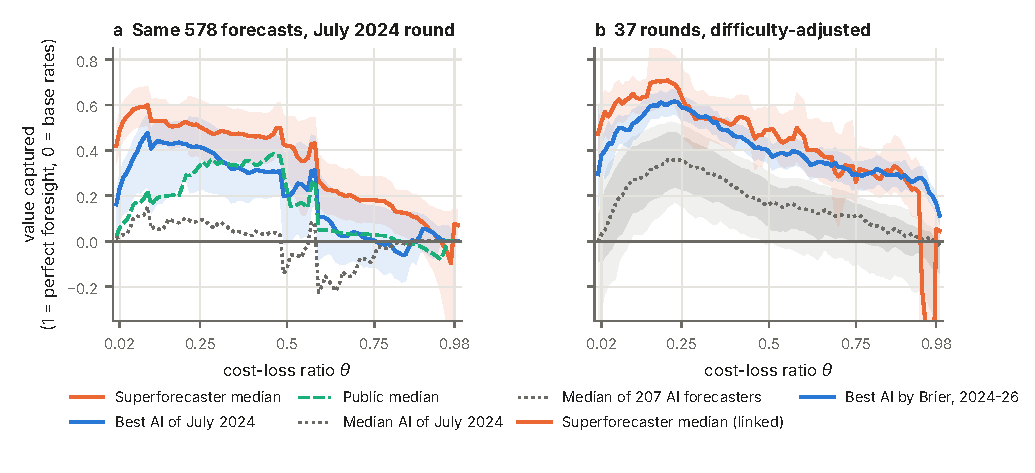
\includegraphics[width=\textwidth]{../figs/fig1_value_curves.pdf}
\vspace{-1.6em}
\caption{Value captured at each cost-loss ratio $\theta$ (the user acts when the forecast exceeds $\theta$). 1 is perfect foresight, 0 is acting on source base rates, below 0 is worse than ignoring the forecaster. \textbf{a:} identical forecasts, July 2024 round, no difficulty adjustment; the best AI is re-selected by Brier score in each bootstrap draw. \textbf{b:} all rounds, difficulty-adjusted; the superforecaster curve is linked to later rounds through the fixed-effects model and rests on their 578 forecasts from 2024. Shaded bands around lines are 95\% question-level bootstrap intervals; grey bands show the spread across AI forecasters (middle 50\% and 80\%).}
\label{fig:curves}
\end{figure}

\begin{table}[!ht]
\centering\small
\caption{The leaderboard in decision units: oracle-equivalent decisions per 100 ($100\,\V$, difficulty-adjusted, dataset and market questions equally weighted) for four user profiles. Grey numbers are ranks among the \nCand{} AI forecasters with at least 2,000 dataset and 200 market forecasts. Rows are the six best by adjusted Brier score. $^\dagger$Human medians are from the July 2024 round only and are linked by the difficulty model.}
\label{tab:profiles}
\begin{tabular}{@{}lrrrrr@{}}
\toprule
& Adj. & Uniform & Precaution & High bar & Even stakes\\
Forecaster & Brier & (= Brier) & ($\bar\theta=0.1$) & ($\bar\theta=0.9$) & ($\bar\theta=0.5$)\\
\midrule
Superforecaster median$^\dagger$ & 0.098 & 49 & 62 & 22 & 48 \\
\addlinespace
Google DeepMind / Gemini & 0.107 & 44 \textcolor{black!55}{(1)} & 53 \textcolor{black!55}{(1)} & 29 \textcolor{black!55}{(1)} & 41 \textcolor{black!55}{(1)} \\
ForecastBench / gpt-5.6-sol (search, code; shown price) & 0.111 & 42 \textcolor{black!55}{(2)} & 50 \textcolor{black!55}{(5)} & 24 \textcolor{black!55}{(2)} & 40 \textcolor{black!55}{(3)} \\
ForecastBench / gpt-5.6-sol (search, code) & 0.113 & 41 \textcolor{black!55}{(3)} & 50 \textcolor{black!55}{(6)} & 17 \textcolor{black!55}{(13)} & 40 \textcolor{black!55}{(2)} \\
Artificial Judgement / aj-v1.5 & 0.113 & 41 \textcolor{black!55}{(4)} & 53 \textcolor{black!55}{(2)} & 18 \textcolor{black!55}{(11)} & 38 \textcolor{black!55}{(4)} \\
Artificial Judgement / aj-v1 & 0.115 & 40 \textcolor{black!55}{(5)} & 51 \textcolor{black!55}{(3)} & 21 \textcolor{black!55}{(5)} & 37 \textcolor{black!55}{(5)} \\
Anthral Labs / blf-ensemble-opus45-gpt55 & 0.116 & 40 \textcolor{black!55}{(6)} & 49 \textcolor{black!55}{(7)} & 23 \textcolor{black!55}{(3)} & 36 \textcolor{black!55}{(6)} \\
\addlinespace
Median of 207 AI forecasters & -- & 20 & 26 & 6 & 18 \\
Public median$^\dagger$ & 0.134 & 31 & 34 & 8 & 33 \\
\bottomrule

\end{tabular}
\end{table}

\subsection{Brier rank predicts decision value, except for high-bar decisions on dataset questions}\label{sec:rank}
Across the \nCand{} forecasters, the Brier ranking correlates \rhoEven{} with the even-stakes ranking, \rhoPre{} with precaution and \rhoHigh{} with high bar; a forecaster moves a median of \moveHigh{} places between the Brier and high-bar rankings, and \keepHigh{} of the Brier top 20 remain in the high-bar top 20 (\keepPre{} for precaution). The top-ranked system is the same under all four profiles (Table~\ref{tab:profiles}), but the systems ranked third and fourth by Brier score fall to 13th and 11th for high-bar users.

The selection experiment (Figure~\ref{fig:selection}) shows how much of this is real. On dataset questions at $\theta=0.3$, past Brier score predicts held-out value almost as well as past value at that threshold does (rank correlation \rhoBMid{} against \rhoOMid). As $\theta$ rises the two separate: at $\theta=0.9$ the Brier ranking's correlation with held-out value is \rhoBNinety{} while the threshold's own record still achieves \rhoONinety; at $\theta=0.95$ it is \rhoBNinetyFive{} against \rhoONinetyFive. Skill at high thresholds is therefore a stable property of forecasters that the Brier score does not see. It has consequences: at $\theta=0.9$ the five forecasters with the best Brier scores deliver \pickB\% of oracle value on held-out dataset questions, while the five with the best record at that threshold deliver \pickO\%, a difference of \pickDiff, with the threshold-specific pick ahead in \pickPOwn\% of splits. The result holds in the wider set of \nCandWide{} forecasters (\pickDiffWide).

Elsewhere the Brier ranking holds up, and this is a finding in its own right. On market questions, where there are a tenth as many items, the Brier ranking predicts held-out value at $\theta=0.5$ slightly better than the threshold's own record (\rhoBMarket{} against \rhoOMarket) and its top-five pick does better on average at \brierWinsMarket{} of \nSelThetas{} thresholds. On the combined score, choosing the single best forecaster by Brier score beats choosing by the user's own threshold at \brierWinsOverall{} of \nSelThetas{} thresholds, and for the precaution and even-stakes profiles the two choices deliver the same value within a point (\selPreB{} against \selPreO; \selEvenB{} against \selEvenO). The Brier score pools information across thresholds, and that lower variance usually outweighs its mismatch with any one user.

\begin{figure}[!ht]
\centering
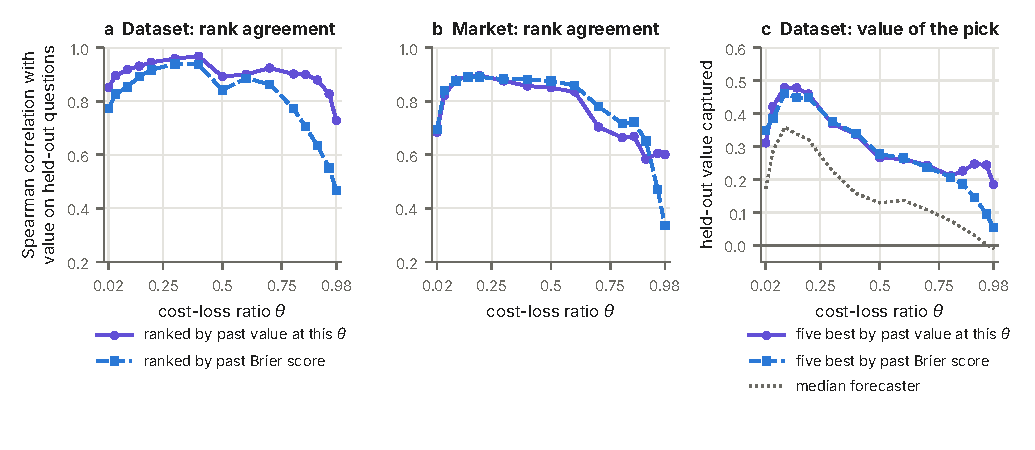
\includegraphics[width=\textwidth]{../figs/fig2_selection.pdf}
\vspace{-1.6em}
\caption{Does past Brier score predict future decision value? Questions are split in half \nSplits{} times; \nCand{} AI forecasters are ranked on one half and evaluated on the other. \textbf{a, b:} rank correlation between each ranking and held-out value at $\theta$. \textbf{c:} held-out value of the five forecasters chosen by each ranking, dataset questions. Points are means over splits.}
\label{fig:selection}
\end{figure}

\subsection{The gaps are not a calibration artefact, and the market price is hard to beat}
If AI forecasters failed in the tails only because they hedge, a monotone recalibration learned from their own track record would restore the value. It does not (Figure~\ref{fig:recal}a,b). On dataset questions recalibration raises the median forecaster's value by \recalGainUni{} points under the uniform profile, \recalGainPre{} under precaution and \recalGainHigh{} under high bar; the median Brier score moves from \recalBrierRaw{} to \recalBrierCal. The share of forecasters no better than base rates at $\theta=0.9$ falls from \dsNonposNinetyRaw\% to \dsNonposNinetyCal\%. The deficit is mostly one of discrimination: these systems do not separate near-certain events from merely likely ones. The median forecaster places only \shareGeNinety\% of its dataset forecasts at or above 0.90.

On market questions the natural comparison is the market price (Figure~\ref{fig:recal}c). The price on the due date captures \priceValue\% of oracle value under the uniform profile; the median AI forecaster captures \medMarketValue\%. Only \beatPriceCount{} of \nCand{} forecasters (\beatPriceShare\%) deliver more value than the price, and no more than \beatPriceMax\% under any profile. This restates in decision terms the Brier-score result of \cite{dominus2026}, with the same caveat: forecasters shown a price saw it ten days before the due date. For a user with access to the market, most AI forecasters on these questions subtract value at every threshold.

\begin{figure}[!ht]
\centering
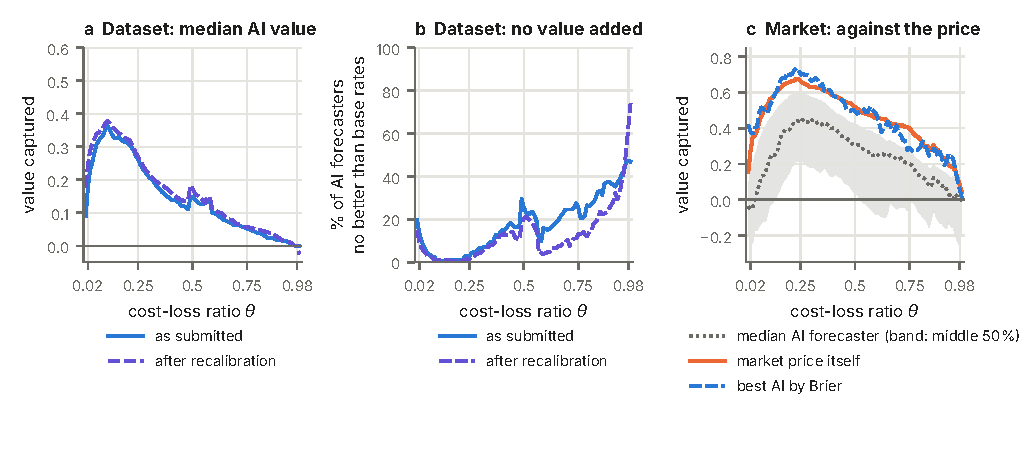
\includegraphics[width=\textwidth]{../figs/fig3_recalibration_price.pdf}
\vspace{-1.6em}
\caption{\textbf{a, b:} Each of \nCand{} AI forecasters is recalibrated by isotonic regression fitted on other questions and re-scored on its own dataset items. Recalibration barely moves the median value curve (a) or the share of forecasters adding no value (b). \textbf{c:} On market questions (difficulty-adjusted), the market price on the due date captures more value than the median AI forecaster at every threshold.}
\label{fig:recal}
\end{figure}

\subsection{``Parity'' depends on who is asking}
Under the uniform profile the superforecaster median captures \oedSuperUni\% of oracle value and the best AI forecaster \oedBestUni\%; the difference, \linkDiffUni, is not distinguishable from zero, consistent with the parity reading of the leaderboard \cite{fri2026}. For precautionary users the superforecasters capture \oedSuperPre\% and the best AI \oedBestPre\%, a difference of \linkDiffPre, with superforecasters ahead in \linkPPre\% of bootstrap draws. For high-bar users the sign reverses, \linkDiffHigh, though not significantly. The best AI was chosen after the fact as the top of \nCand, which flatters it, so the precaution gap is if anything understated. On identical items in 2024 the superforecasters led the best AI under every profile, with intervals excluding zero for three of the four (uniform: \rOneDiffUni; precaution: \rOneDiffPre; high bar: \rOneDiffHigh). The users for whom AI has caught up are those with moderate thresholds; those guarding against unlikely, costly events are still better served by the human panel.

\subsection{Leaderboard intervals are too narrow}
The leaderboard's bootstrap resamples question-horizon items within a round. Dataset questions contribute \dePer{} items each on average (several horizons, recurring across rounds), and their outcomes are dependent. Holding question effects fixed in both cases, resampling underlying questions instead of items widens the standard error of the adjusted dataset Brier score by a median factor of \deRatio{} (interquartile range \deLo{} to \deHi; wider for \deShare\% of forecasters). Claims that two entries are distinguishable should be read with intervals about that much wider.

\section{Discussion and Limitations}
\textbf{Implications.} (1) For most users the Brier leaderboard picks the right forecasters; it is a low-variance summary and should not be replaced by threshold-specific rankings. What it conceals is the \emph{level}: a forecaster ranked high can still deliver almost nothing to users at the extremes. Benchmarks could publish the value curve, or at least a precaution and a high-bar score, next to the Brier score at no extra data cost. (2) High-threshold skill on dataset questions is real, persistent and invisible to the Brier score. Systems meant for decisions that require near-certainty should be selected on it directly. (3) Parity claims should name the user. Many safety-relevant decisions are cheap precautions against rare and costly events, and that is the region where AI forecasters trail superforecasters and where the typical one adds least. (4) As a candidate ``QALY for epistemics'', value captured is anchored, additive over decisions, comparable across domains with different base rates, and computable from any set of resolved binary forecasts.

\textbf{Limitations.} Forecasting questions are not decisions: we assign every question the same hypothetical user, binary actions and risk neutrality, and real users' thresholds vary across questions. Value is relative to in-sample source base rates, a reference that is slightly too strong. The human comparison in the pooled analysis rests on 578 forecasts from 2024 and on the additive difficulty model, which is least trustworthy in the tails and for market questions (57 human forecasts). Forecaster identities are file-level names rather than the leaderboard's normalised identities, so some systems are split across variants. The market price used for adjustment postdates the price shown to forecasters. Recalibration is cross-fitted by question, not by time. The selection experiment holds question effects fixed across halves. Further limitations and dual-use considerations are in Appendix~\ref{app:limits}.

\textbf{Future work.} Elicit real thresholds from decision-makers and weight by them; extend to multi-action and continuous decisions; track value curves at each model release; test whether training on a tail-weighted proper score moves high-threshold skill.

\section{Conclusion}
A Brier score is an answer to ``how good are these forecasts for the average of all possible users?'' We asked the question for particular users. On \nForecastsM{} million resolved forecasts, the Brier ranking turns out to be a better guide to decision value than its critics might expect and, for most thresholds, at least as good as rankings built for the purpose. But it fails for high-bar decisions on dataset questions, it hides how little value most AI forecasters deliver at extreme stakes or beyond the market price, and it makes ``parity with superforecasters'' sound like one fact when it is several. Reporting value captured by threshold costs nothing beyond data benchmarks already collect and tells a decision-maker whether a forecaster is of use to them.

\section*{Code and Data}
Code: \url{https://github.com/gavenren/decision-value-audit}. The analysis is a small Python package (\texttt{oed}) with 18 unit tests covering the scoring identities, the fixed-effects solver and the resampling; one command rebuilds every number, table and figure in this report from the public ForecastBench files. All of the code was written during the sprint. Data: ForecastBench datasets repository (commit of 11 November 2026) and processed forecast sets (downloaded 13 November 2026), CC BY-SA 4.0 \cite{karger2025}. No information hazards.

\section*{Author Contributions}
Gaven Ren is the sole author.

\begin{thebibliography}{99}\small
\setlength{\itemsep}{.1ex}
\bibitem{karger2025} Karger, E., Bastani, H., Yueh-Han, C., Jacobs, Z., Halawi, D., Zhang, F., Tetlock, P.\,E. (2025). ForecastBench: A dynamic benchmark of AI forecasting capabilities. \emph{ICLR 2025}. \url{https://arxiv.org/abs/2409.19839}. Data: \url{https://github.com/forecastingresearch/forecastbench-datasets}; code: \url{https://github.com/forecastingresearch/forecastbench}.
\bibitem{fri2026} Forecasting Research Institute (2026). AI models have likely reached parity with superforecasters on ForecastBench. 16 July 2026. \url{https://forecastingresearch.substack.com/p/ai-models-have-likely-reached-parity}
\bibitem{schervish1989} Schervish, M.\,J. (1989). A general method for comparing probability assessors. \emph{Annals of Statistics} 17(4), 1856--1879.
\bibitem{ehm2016} Ehm, W., Gneiting, T., Jordan, A., Kr\"uger, F. (2016). Of quantiles and expectiles: consistent scoring functions, Choquet representations and forecast rankings. \emph{Journal of the Royal Statistical Society B} 78(3), 505--562. \url{https://arxiv.org/abs/1503.08195}
\bibitem{murphy1977} Murphy, A.\,H. (1977). The value of climatological, categorical and probabilistic forecasts in the cost-loss ratio situation. \emph{Monthly Weather Review} 105(7), 803--816.
\bibitem{richardson2000} Richardson, D.\,S. (2000). Skill and relative economic value of the ECMWF ensemble prediction system. \emph{Quarterly Journal of the Royal Meteorological Society} 126(563), 649--667. \url{https://doi.org/10.1002/qj.49712656313}
\bibitem{goodjudgment2026} Good Judgment (2026). What ForecastBench doesn't measure (yet). 14 April 2026. \url{https://goodjudgment.substack.com/p/what-forecastbench-doesnt-measure}
\bibitem{dominus2026} Dominus (2026). The copier line: what ForecastBench's market scores actually measure. EA Forum, August 2026. \url{https://forum.effectivealtruism.org/posts/8YuG9EuhyYqaNBt7F/the-copier-line-what-forecastbench-s-market-scores-actually}
\bibitem{liptay2026} Liptay, T. (2026). Our correlation weights for ForecastBench's Oct 25 round. FutureSearch, 26 October 2026. \url{https://futuresearch.ai/blog/forecastbench-correlation-weights/}
\bibitem{yang2026} Yang, Q., Mahns, S., Li, S., Gu, A., Wu, J., Xu, H. (2026). LLM-as-a-Prophet: Understanding predictive intelligence with Prophet Arena. \emph{ICLR 2026}. \url{https://arxiv.org/abs/2510.17638}
\bibitem{dimitriadis2024} Dimitriadis, T., Gneiting, T., Jordan, A.\,I., Vogel, P. (2024). Evaluating probabilistic classifiers: the triptych. \emph{International Journal of Forecasting} 40(3), 1101--1122. \url{https://arxiv.org/abs/2301.10803}
\bibitem{buja2005} Buja, A., Stuetzle, W., Shen, Y. (2005). Loss functions for binary class probability estimation and classification: structure and applications. Working paper, University of Pennsylvania. \url{https://sites.stat.washington.edu/wxs/Learning-papers/paper-proper-scoring.pdf}
\bibitem{merkle2013} Merkle, E.\,C., Steyvers, M. (2013). Choosing a strictly proper scoring rule. \emph{Decision Analysis} 10(4), 292--304. \url{https://doi.org/10.1287/deca.2013.0280}
\bibitem{kalai2025} Kalai, A.\,T., Nachum, O., Vempala, S.\,S., Zhang, E. (2025). Why language models hallucinate. \url{https://arxiv.org/abs/2509.04664}
\bibitem{state2026} Ben N, Csaky, A. (2026). State of the field: AI for epistemics and coordination. LessWrong. \url{https://www.lesswrong.com/posts/uw8RQ8yjKexnhTw6E/state-of-the-field-ai-for-epistemics-and-coordination}
\bibitem{dimitriadis2021} Dimitriadis, T., Gneiting, T., Jordan, A.\,I. (2021). Stable reliability diagrams for probabilistic classifiers. \emph{PNAS} 118(8), e2016191118. \url{https://doi.org/10.1073/pnas.2016191118}
\end{thebibliography}

\appendix
\section{Limitations and Dual-Use / Ethical Considerations}\label{app:limits}
\textbf{What the results establish.} On ForecastBench's binary questions, under a cost-loss decision model with a single threshold per user, (i) Brier rank is a reliable guide to held-out decision value for moderate thresholds and an unreliable one for high thresholds on dataset questions; (ii) the typical AI forecaster adds little value at extreme thresholds and less than the market price on market questions; (iii) the best AI forecaster is statistically level with the 2024 superforecaster median for uniformly distributed users and behind it for precautionary users.

\textbf{What they do not establish.} They do not show how AI forecasts affect real decisions, since no decisions were observed; the thresholds are hypothetical. They do not show that superforecasters today would lead or trail today's systems on the same questions: the human data are from one round in 2024 and the link to later rounds is a statistical model. They say nothing about questions that are not binary, about forecast updating, or about explanations. ForecastBench's dataset questions are a narrow family (changes in time series and counts), and the high-bar finding is specific to them. Value captured depends on the reference policy; a different reference (for example, a naive time-series model) changes levels, though not the rankings within a question type. Rankings among forecasters with small samples are noisy, which is why the selection experiment uses only those with large ones. The best AI forecaster is selected post hoc.

\textbf{Dual use.} The analysis identifies where forecasters are weak, which a developer could use to tune a system to a published profile rather than to improve it. Tuning to a proper scoring rule is not gaming: every profile score here is strictly proper for binary events, so the optimal response is still to report honest probabilities. A second risk is misuse of the unit as marketing (``captures 44\% of oracle value'') without the threshold, the reference or the interval; we recommend that any such figure be reported with all three. We see no route by which this work helps manipulation or deception.

\textbf{Personal data.} None was used. The human forecasts enter only as the published per-question medians of the superforecaster and public panels; we did not use individual-level responses, identifiers or rationales in any reported result.

\section{Details}\label{app:details}
\textbf{Brier identity.} For $y=1$, $2\int_0^1 r_\theta\,d\theta=2\int_p^1(1-\theta)\,d\theta=(1-p)^2$; for $y=0$, $2\int_0^p\theta\,d\theta=p^2$.

\textbf{Closed-form profile scores.} For $w$ the Beta$(a,b)$ density and $I_x$ the regularised incomplete beta function,
$\int_0^1 w(\theta)\,r_\theta(p,y)\,d\theta=(1-y)\,\tfrac{a}{a+b}\,I_p(a+1,b)+y\,\tfrac{b}{a+b}\,\bigl(1-I_p(a,b+1)\bigr)$. With $a=b=1$ this is half the Brier score. The unit tests check the formula against numerical integration and check the fixed-effects solver against dense least squares.

\textbf{Reference policy.} Source base rates are pooled over all scored items of all rounds: ACLED 0.11, DBnomics 0.58, FRED 0.48, Wikipedia 0.21, Yahoo Finance 0.57, INFER 0.11, Kalshi 0.47, Manifold 0.34, Metaculus 0.23, Polymarket 0.23.

\textbf{Departures from the leaderboard.} (i) Question effects for dataset questions are fitted on all non-dummy forecasters. (ii) Forecasters are identified by team and model name as written in each file. (iii) Only binary resolutions are scored; all resolved items in the snapshot are binary. (iv) The bootstrap resamples underlying questions and holds question effects fixed. (v) Where one forecaster name appears twice on an item within a round (0.03\% of rows), the first file is kept.

\section*{LLM Usage Statement}
The analysis code, tests, figures and the text of this report were drafted by Claude (Anthropic), an AI model, at the author's direction during the sprint: the author set the task and supplied the ForecastBench archive; the model proposed the project, wrote and ran the code, and wrote the draft. Every number in the report is generated from the analysis output by script rather than typed by hand, and every reference was checked against its source.

\end{document}
